  \documentclass[11pt]{article}

  \usepackage{fullpage}
  \usepackage{graphicx}
  \graphicspath{ {./images/} }
  \begin{document}

  \title{ARM Checkpoint Report}
  \author{Otto White, Paulo Lemos, Robert Stock, Weizhong Zhao}

  \maketitle

  \section*{Group Organisation}

  \subsection*{How we split the work}

After reviewing the specification together, we decided to split the emulator task into three  sections: creating general file and program structure, loader and fetch-decode-execute functions, and the four ARM instructions. We worked on setting programming standards and general program/file structure as a group as this would form the basis of our entire emulator. Next, we allocated the loader and fetch functions to one pair (Weizhong and Paulo) and the decode and execute functions to another (Otto and Rob). The final four instructions were distributed to each member as follows: data processing to Otto, multiply to Rob, single data transfer to Paulo and branch to Weizhong. Once all were completed, we came together to merge our seperate branches. Debugging and final testing was then performed by Otto.

  \subsection*{How well the group is working}

For the majority of the emulator work, communication was carried out through online meetings and messaging due to schedule and location differences. Despite this, we were still able to work efficiently as we had set up internal deadlines and allocated tasks early on. By working on general program structure and writing reusable code such as definitions.h together, each of us benefited from having a strong understanding of the emulator as a whole and how different parts fit together. We distributed tasks by function but we quickly realised that some parts were more complicated than others which resulted in varying amounts of workload. For the assembler, we plan to be more flexible and let those who finish their tasks earlier help with others. While pair programming was useful in ensuring code correctness, we found it slower than solo programming which we plan to do for most of the assembler. To compensate for no longer pair programming, we will create a comprehensive testing system for our assembler (more details below). Overall, we feel our group has been working well and completing objectives in a timely manner.

  \section*{Implementation Strategies}

  \subsection*{Emulator structure}

Our emulator is structured as pictured below. At the top level we have the emulate.c file which runs the main process. In this file the instructions are loaded using the loader.c script and then run on the pipeline.c script. The state is also instantiated and passed by pointer to the pipeline. The pipeline.c script runs the execute, decode and fetch stages - in that order, where the next stage is processing the next instruction. The fetch stage passes a pointer to the state into the fetch.c script, which then fetches the next instruction and returns it as a 32 bit binary number. The decode stage passes a pointer to the state to the decode.c script, and the 32 bit binary instruction to be decoded. This then translates it into an Instruction struct, which is returned. The execute phase passes a pointer to the state and a pointer to the Instruction struct into the execute.c script. This then checks the type of instruction and then passes both a pointer to the instruction struct and a pointer to the state to one of the four instructions. These are handled by the data_processing.c, multiply.c, single_data_transfer.c or the branch.c scripts. These are all defined in the instructions.h file, which is included in the pipeline.c script. All the files also rely on the definitions.h file to define the State struct, Instruction struct as well as the Instruction_type, Opcode, and Condition enums, which are used in the Instruction struct.

 \begin{figure}[h]
 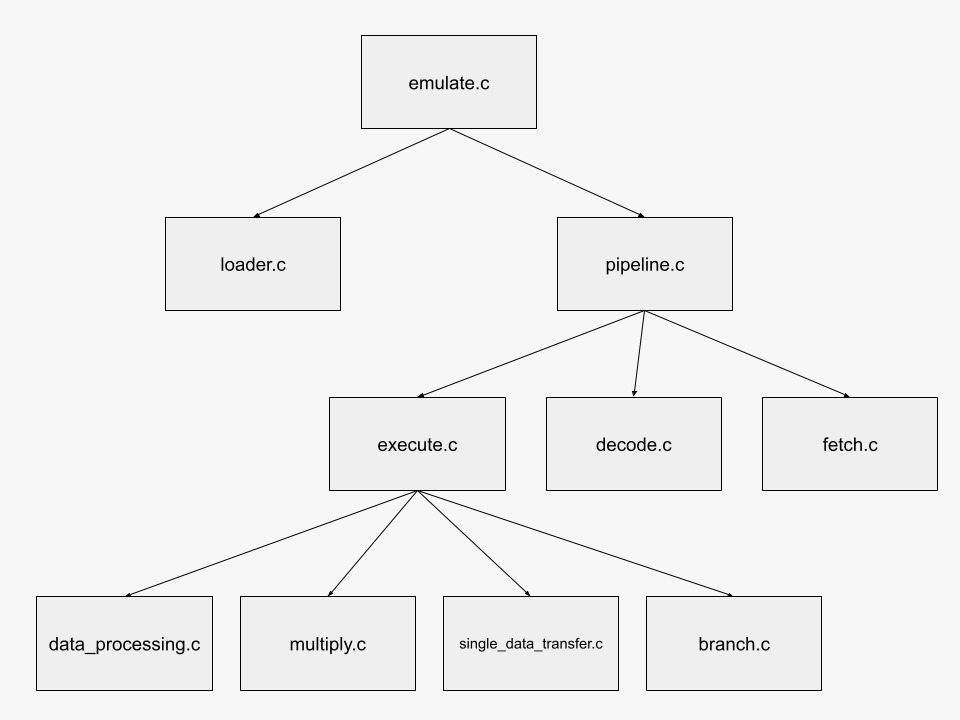
\includegraphics[scale=0.4]{emulator_structure}
 \centering
 \end{figure}

  \end{document}
